\subsubsection{UC\theuccount-GP - Rimozione utente dal sistema}
		\begin{figure}[H]
			\centering
				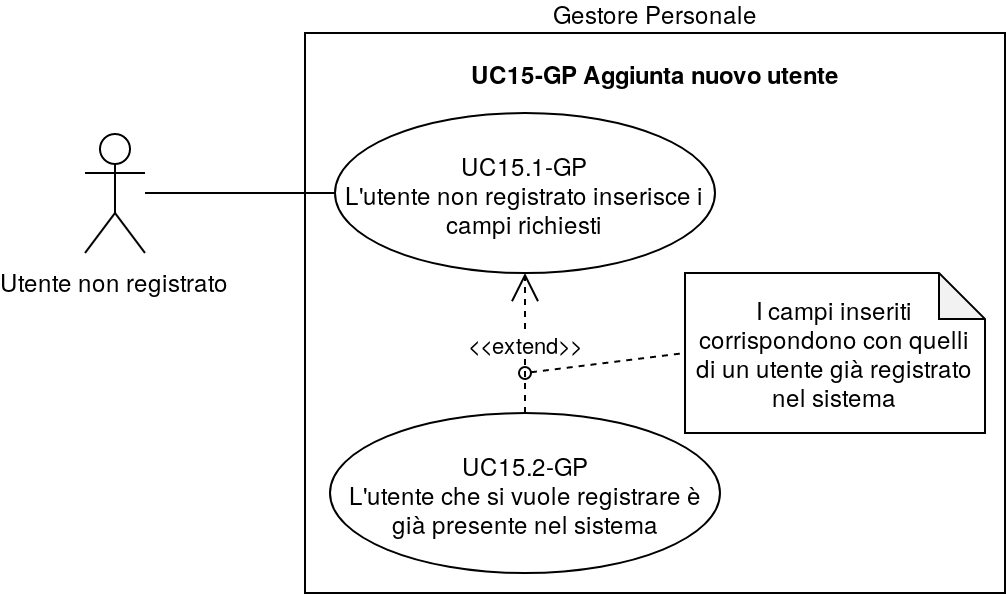
\includegraphics[width=\columnwidth]{img/casi_d'uso/UC15.png}\\
			\caption{UC\theuccount-GP - Rimozione utente dal sistema}
		\end{figure}
	\begin{itemize}
		\item \textbf{Codice}: UC\theuccount-GP.
		\item \textbf{Titolo}: rimozione utente dal sistema.
		\item \textbf{Attori primari}: utente.
		\item \textbf{Descrizione}: l'utente rimuove l'utente selezionato dal sistema.
		\item \textbf{Precondizione}: un utente già presente nel sistema deve essere rimosso.
		\item \textbf{Postcondizione}: un utente viene rimosso dal sistema.
		\item \textbf{Scenario principale}:
		\begin{enumerate}
			\item L'utente rimuove l'utente selezionato
		\end{enumerate}
\end{itemize}
	
	\stepcounter{subuccount}
	\subsubsection{UC\theuccount.\thesubuccount-GP - Rimozione avvenuta con successo}
		\begin{figure}[H]
			\centering
			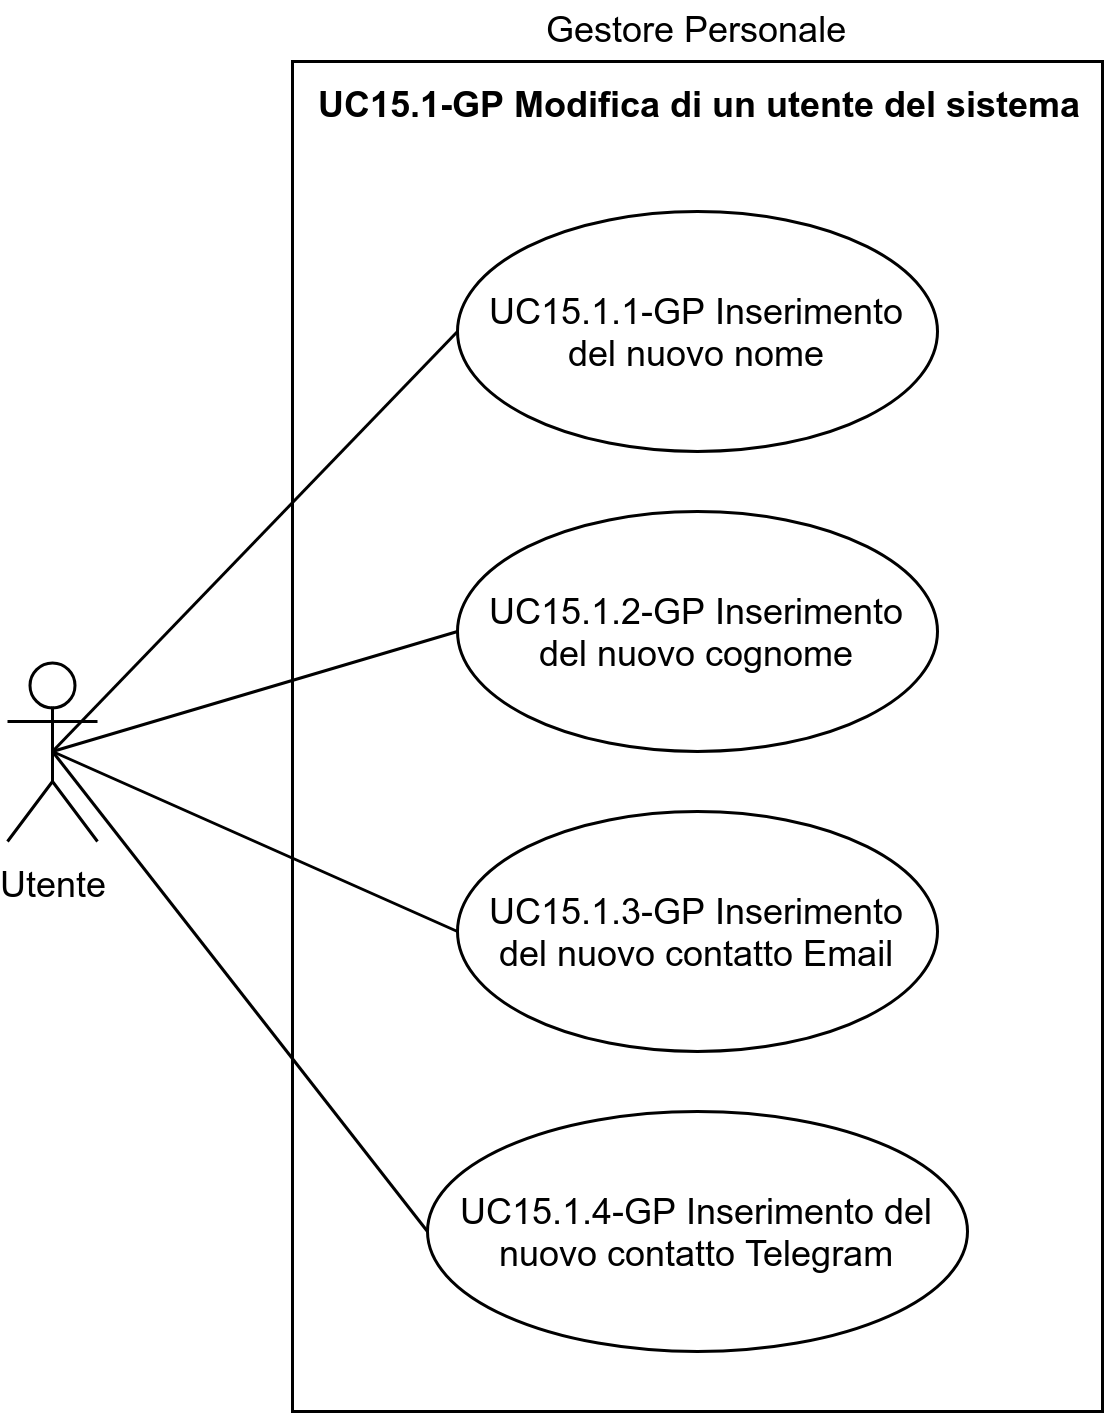
\includegraphics[width=0.6\columnwidth]{img/casi_d'uso/UC15_1.png}\\
			\caption{UC\theuccount.\thesubuccount-GP - Rimozione avvenuta con successo}
		\end{figure}
		\begin{itemize}
			\item \textbf{Codice}: UC\theuccount.\thesubuccount-GP.
			\item \textbf{Titolo}: rimozione avvenuta con successo.
			\item \textbf{Attori primari}: utente.
			\item \textbf{Descrizione}: un utente, acceduto al sistema, rimuove un altro utente presente nel sistema tramite l'inserimento del suo contatto Email o Telegram.
			%il contatto Email o Telegram dell'utente da rimuovere è presente nel sistema, per cui la rimozione avviene con successo.
			\item \textbf{Precondizione}: un utente già presente nel sistema deve essere rimosso.
			\item \textbf{Postcondizione}: un utente con il contatto Email o Telegram inserito viene rimosso dal sistema.
			\item \textbf{Scenario principale}:
			\begin{enumerate}
				\item L'utente inserisce ciò che è richiesto dal sistema
				\item L'utente conferma l'invio dei dati
				\item L'utente da rimuovere è stato rimosso dal sistema
			\end{enumerate}
			\item \textbf{Estensioni}:
			\begin{itemize}
				\item Errore contatto non presente nel sistema [UC\theuccount.2-GP]
				\item L'utente vuole rimuovere se stesso [UC\theuccount.3-GP]
			\end{itemize}
		\end{itemize}
			
			\stepcounter{subsubuccount}
			\subsubsection{UC\theuccount.\thesubuccount.\thesubsubuccount-GP - Inserimento contatto Email}
				
				\begin{itemize}
					\item \textbf{Codice}: UC\theuccount.\thesubuccount.\thesubsubuccount-GP.
					\item \textbf{Titolo}: inserimento contatto Email.
					\item \textbf{Attori primari}: utente.
					\item \textbf{Descrizione}: l'utente ha aggiunto il contatto Email relativo all'utente che vuole rimuovere.
					\item \textbf{Precondizione}: un utente già presente nel sistema deve essere rimosso.
					\item \textbf{Postcondizione}: il contatto dell'utente da rimuovere Email è stato inserito.
					\item \textbf{Scenario principale}:
					\begin{enumerate}
						\item L'utente inserisce il contatto Email dell'utente da rimuovere
					\end{enumerate}
				\end{itemize}
			
			\stepcounter{subsubuccount}
			\subsubsection{UC\theuccount.\thesubuccount.\thesubsubuccount-GP - Inserimento contatto Telegram}
				
				\begin{itemize}
					\item \textbf{Codice}: UC\theuccount.\thesubuccount.\thesubsubuccount-GP.
					\item \textbf{Titolo}: inserimento contatto Telegram.
					\item \textbf{Attori primari}: utente.
					\item \textbf{Descrizione}: l'utente ha aggiunto il contatto Telegram relativo all'utente che vuole \newline rimuovere.
					\item \textbf{Precondizione}: un utente già presente nel sistema deve essere rimosso.
					\item \textbf{Postcondizione}: il contatto Telegram dell'utente da rimuovere è stato inserito.
					\item \textbf{Scenario principale}:
					\begin{enumerate}
						\item L'utente inserisce il contatto Telegram del utente da rimuovere.
					\end{enumerate}
				\end{itemize}
			
			\stepcounter{subuccount}
			\subsubsection{UC\theuccount.\thesubuccount-GP - Errore contatto non presente nel sistema}
					
				\begin{itemize}
					\item \textbf{Codice}: UC\theuccount.\thesubuccount-GP.
					\item \textbf{Titolo}: errore contatto non presente nel sistema.
					\item \textbf{Attori primari}: utente.
					\item \textbf{Descrizione}: l’utente viene avvisato che il contatto inserito non è presente nel sistema.
					\item \textbf{Precondizione}: un utente già presente nel sistema deve essere rimosso.
					\item \textbf{Postcondizione}: il sistema comunica all’utente che utilizza il sistema l’errore e nessun utente viene rimosso.
					\item \textbf{Scenario principale}:
					\begin{enumerate}
						\item L'utente selezionato attraverso il contatto Telegram o Email non viene rimosso perché non presente nel sistema.
					\end{enumerate}
				\end{itemize}
			
			\stepcounter{subuccount}
			\subsubsection{UC\theuccount.\thesubuccount-GP - L'utente rimuove se stesso dal sistema}
			
			\begin{itemize}
				\item \textbf{Codice}: UC\theuccount.\thesubuccount-GP.
				\item \textbf{Titolo}: l'utente rimuove se stesso dal sistema.
				\item \textbf{Attori primari}: utente.
				\item \textbf{Descrizione}:  l’utente inserisce il proprio identificativo per rimuoversi dal sistema.
				\item \textbf{Precondizione}: un utente già presente nel sistema deve essere rimosso.
				\item \textbf{Postcondizione}: l'utente non risulta più acceduto al sistema che non riconosce più l'utente ormai rimosso.
				\item \textbf{Scenario principale}:
				\begin{enumerate}
					\item L'utente selezionato attraverso il contatto Telegram o Email viene rimosso dal sistema.
					\item L'utente viene automaticamente fatto uscire dall'applicazione.
					%TODO: aggiungere un caso include perchè se l'utente è rimosso allora => l'utente viene fatto uscire dal sistema?
				\end{enumerate}
			\end{itemize}